\documentclass[11pt,openright,a4paper]{report}
%%
%% This document template assumes you will use pdflatex.  If you are using
%% latex and dvipdfm to translate to pdf, insert dvipdfm into the options.
%%
%%
%% Package includes to provide the basic style
%%
\usepackage{harvard}    % Uses harvard style referencing
\usepackage{graphicx}   % Permits import of various graphics formats
\usepackage{hyperref}   % Provides hyperlinks to sections automatically
\usepackage{pdflscape}  % Provides landscape mode for end code listings
\usepackage{multicol}   % Provides ability to split output into columns
\usepackage{listings}   % Provides styled code listings
\usepackage{hyperref}   % Provides URL stuff
\usepackage{nameref}    % Reference chapter names
\usepackage{enumitem}   % Better list control
\usepackage{mathtools}  % Equations

%%
%% Set some page size changes from the standard article class
%%
\usepackage{calc}
\setlength{\parskip}{6pt}
\setlength{\parindent}{0pt}
\addtolength{\hoffset}{-0.5cm}
\addtolength{\textwidth}{2.5cm}


%%
%% Format definitions for the style
%%
\bibliographystyle{agsm}  %{alpha}
\citationstyle{dcu}
\pagestyle{headings}
\fussy


%%
%% Definitions to provide layout in the dissertation title pages
%%
\newenvironment{spaced}[1]
  {\begin{minipage}[c]{\textwidth}\vspace{#1}}
  {\end{minipage}}


\newenvironment{centrespaced}[2]
  {\begin{center}\begin{minipage}[c]{#1}\vspace{#2}}
  {\end{minipage}\end{center}}


\newcommand{\declaration}[2]{
  \thispagestyle{empty}
  \begin{spaced}{4em}
    \begin{center}
      \LARGE\textbf{#1}
    \end{center}
  \end{spaced}
  \begin{spaced}{3em}
    \begin{center}
      Submitted by: #2
    \end{center}
  \end{spaced}
  \begin{spaced}{5em}
    \section*{COPYRIGHT}

    Attention is drawn to the fact that copyright of this dissertation rests
    with its author. The Intellectual Property Rights of the products
    produced as part of the project belong to the author unless otherwise specified
    below, in accordance with the University of Bath's policy on intellectual property
   (see http://www.bath.ac.uk/ordinances/22.pdf).

    This copy of the dissertation has been supplied on condition that anyone
    who consults it is understood to recognise that its copyright rests with its
    author and that no quotation from the dissertation and no information
    derived from it may be published without the prior written consent of
    the author.

    \section*{Declaration}
    This dissertation is submitted to the University of Bath in accordance
    with the requirements of the degree of Bachelor of Science in the
    Department of Computer Science. No portion of the work in this dissertation
    has been submitted in support of an application for any other degree
    or qualification of this or any other university or institution of learning.
    Except where specifically acknowledged, it is the work of the author.
  \end{spaced}

  \begin{spaced}{5em}
    Signed:
  \end{spaced}
  }


\newcommand{\consultation}[1]{%
\thispagestyle{empty}
\begin{centrespaced}{0.8\textwidth}{0.4\textheight}
\ifnum #1 = 0
This dissertation may be made available for consultation within the
University Library and may be photocopied or lent to other libraries
for the purposes of consultation.
\else
This dissertation may not be consulted, photocopied or lent to other
libraries without the permission of the author for #1
\ifnum #1 = 1
year
\else
years
\fi
from the date of submission of the dissertation.
\fi
\vspace{4em}

Signed:
\end{centrespaced}
}


% Code listing without page breaks
\lstnewenvironment{Code}[1][]%
  {\minipage{\linewidth}
   \lstset{basicstyle=\ttfamily\footnotesize,frame=single,#1}}
  {\endminipage}

%%
%% END OF DEFINITIONS
%%

    %% These are the includes required for the doc

\newcommand\myTitle{Extending a StarCraft AI Behaviour Library}
\newcommand\myAuthor{Alex Aiton}

% Give description lists an indent
\setdescription{leftmargin=1cm,labelindent=1cm}

\title{\myTitle}
\author{\myAuthor}
\date{Bachelor of Science in Computer Science with Honours\\The University of Bath\\April 2014}


\begin{document}


% Set this to the language you want to use in your code listings (if any)
\lstset{language=Java,breaklines,breakatwhitespace,basicstyle=\small}


\setcounter{page}{0}
\pagenumbering{roman}


\maketitle
\newpage


% Set this to the number of years consultation prohibition, or 0 if no limit
\consultation{0}
\newpage


\declaration{\myTitle}{\myAuthor}
\newpage


\abstract
Your abstract should appear here.  An abstract is a short
paragraph describing the aims of the project, what was
achieved and what contributions it has made.
\newpage


\tableofcontents
\newpage
\listoffigures
\newpage
\listoftables
\newpage


\chapter*{Acknowledgements}
Add any acknowledgements here.
\newpage


\setcounter{page}{1}
\pagenumbering{arabic}



\chapter{Introduction}
%% Uncomment this to include a separate tex file wih the introduction contents
%\include{introduction.tex}

This is the introductory chapter.


\chapter{Literature Survey}
In 2012, Simon Davies created an AI agent for the real-time strategy game StarCraft: Brood War. He followed the Behaviour Oriented Design development methodology and focused his efforts on an agent for the Zerg race. This project aims to generalise the work Davies performed to allow for agents of other races and possibly implement improvements.

StarCraft has recently seen increased development in the field of AI, due to the release of a convenient API for the purpose of AI development. Before beginning focused development effort, a survey of the work done in this area was conducted. What follows is the results of this survey, including an explanation of what StarCraft is; the field of AI and agents in general; the Behaviour Oriented Design methodology; an overview of what Davies accomplished; and a review of some techniques that could be used to improve Davies' agent.
\section{StarCraft}
StarCraft is a real-time strategy game where the player commands an army from one of three distinct races\footnote{Races can be thought about as teams or factions. Race is the term used in the StarCraft community}. It was released in 1998 by Blizzard Entertainment and its expansion StarCraft: Brood War was released later the same year \cite{Blizzard}. During a game, the player controls their army from a top-down perspective, or ``God's eye view'' (see figure~\ref{fig:StarCraft}). The army must harvest two limited resources, minerals and vespene gas, and use them to construct buildings, recruit units and research upgrades with the ultimate goal of destroying the opponent. The game can be said to be split into three stages: The opening, where choosing the most suitable order of construction is vital due to limited resources; the mid-game, where players build up for larger attacks and must expand to gain more resources; and the end-game, where one player has gained the advantage and should be looking to make a very large push to secure it \cite{yi2011adaptive}.

The three races differ from each other substantially in both play style and unit ability. The insectile Zerg focus on small, fast and cheap units and swarm tactics; the psychic and advanced Protoss focus on expensive but extremely powerful units; and the human Terran are the balance between the two, not as weak or as numerous as the Zerg, but not as powerful or as expensive as the Protoss. They also focus on attacking from range.  Due to the game's age and popularity, there are many online communities that have collated a large amount of information about the game and effective strategies, such as the \citeasnoun{SCWiki} and \citeasnoun{TeamLiquid}.

StarCraft has regularly found itself used as a subject in academia, probably due to its prominence and well-balanced game play.  Uses can vary from essays on what StarCraft's design communicates \cite{galloway2007starcraft}, analysis of the game's network traffic \cite{dainotti2005packet}, to algorithmically generating playable maps \cite{togelius2010multiobjective}. The creation of the Brood War Application Programming Interface (BWAPI) in 2010 \cite{bwapiMain} has led to increased usage as a platform to explore and construct AI and a target for AI competitions \cite{bwapiCompetitions}.

\begin{figure}[h]
    \centering
    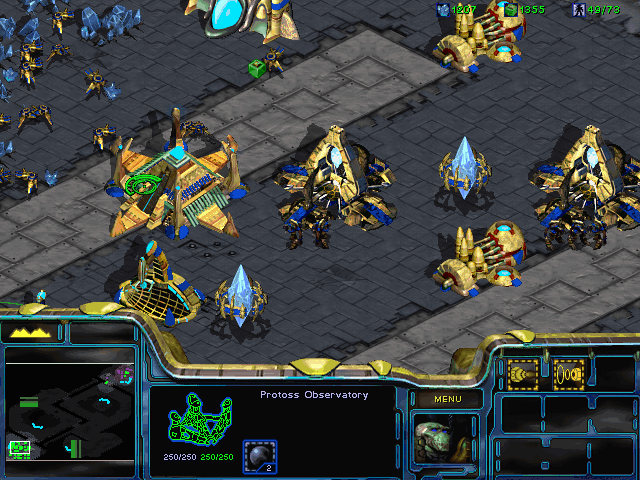
\includegraphics[width=0.8\textwidth,natwidth=640,natheight=480]{StarCraft.png}
    \caption{A screenshot of StarCraft during a game. It shows the base of a Protoss player}
    \label{fig:StarCraft}
\end{figure}

\section{Artificial Intelligence}
AI is a wide ranging field concerned with the research and development of machines/programs capable of intelligence. It includes a wide variety of sub-fields like ``computer vision, natural language, decision theory, genetic algorithms and robotics'' \cite{mccorduck2004machines}. There is the concept of strong AIs, which are the kind of AI visualised by the general public and science fiction writers, true ``machines that think'', conscious and capable of human emotion \cite{kurzweil2005singularity}. AIs that don't attempt to simulate the entirety of human intelligence can be called weak AI, and it's probably safe to say all AI's created to date are weak AI, including those found in games.

The concept of an agent is a popular one in AI. An agent is a system capable of flexible, autonomous action in some environment \cite{wooldridge1995intelligent}. That's a rather vague definition, so to expand it; an agent is a computer system which has a goal to accomplish, resides in an environment which it can effect some change upon and can react to changes in that environment. An environment does not have to be physical, but there are other classifications to consider \cite{russell1995artificial}:
\begin{itemize}
\item{Accessible vs. inaccessible – How much information is available to the agent about the environment? Accessible environments provide complete, accurate and up-to-date information about the environment's state. }
\item{Deterministic vs. non-deterministic – What happens when the agent acts? In deterministic environments an action has a single guaranteed effect, with no uncertainty. }
\item{Static vs. dynamic – Is anything else changing the environment? Static environments only change due to actions by the agent.}
\item{Episodic vs. non-episodic – How is the agent rated? An agent rated in an episodic environment takes part in several discrete episodes which remain independent, so past and future performances aren't important.  For example, an AI taking part in a tournament could consider each game to be a single episode.}
\item{Discrete vs. continuous – How many actions are available to the agent? Discrete environments have a very limited and fixed number actions and a small amount of required knowledge in it.}
\end{itemize}
StarCraft can be argued to be an inaccessible, deterministic, dynamic, continuous environment with the possibility to be episodic and accessible depending on game settings \cite{davies2012}. The majority of StarCraft games have the fog of war setting enabled, so only objects within unit vision are visible and have up-to-date information. It is possible to disable the setting, turning it into an accessible environment. Almost all agent actions are deterministic, though there is some small randomness in ranged attacks. StarCraft is played against another agent, so must be dynamic. The number of units and the number of positions they can be in make it more like a continuous environment than a discrete one, though I think the number of actions available is just extremely high rather than infinite.

\section{Behaviour Oriented Design (BOD)}
\label{BOD}
BOD is an AI development methodology conceived by Bryson \cite{bryson2001intelligence}. It details both an agent architecture and a design methodology.  The BOD architecture has two parts, a modular library of behaviours (actions, senses and state) and parallel rooted, ordered, slip-stack,  and hierarchical (POSH) reactive plans for action selection. The methodology specifies how to decompose an agent's behaviours and emphasises an iterative development approach for implementation \cite{bryson2003behavior}. BOD focuses on the design of the AI system, aiming to produce agents that are easy to extend and maintain. It's modularity allows many different AI techniques to be used in tandem, encouraging the developer to use whatever approach fits an individual problem best \cite{gaudlbehaviour}.

\subsection{Architecture}
As stated,  the BOD architecture consists of two main parts:
\begin{description}
\item[The Behaviour Library] Behaviours are like object oriented design objects and encapsulate how to do something, including perception and actions. Behaviours should be modular, can have state, can implement learning techniques, or even be wrappers for external libraries. This separation from the action selection also facilitates code re-use and allows modification of behaviours without affecting plans \cite{gaudlbehaviour}.
\item[POSH plans and action selection] \label{POSHPlans}POSH plans are a hierarchy of actions and their triggers \cite{gaudlbehaviour}. The primitives of the hierarchy are actions and senses. These primitives are formed into three groupings, action patterns, competences and drive collections, in order of increasing complexity. Action patterns are simple sequences of primitives; competences are basic reactive plans, a prioritised list of actions and triggers; drive collections are the root of the hierarchy and determine where the agent's attention should be focused \cite{bryson2003behavior}.
\end{description}

\subsection{Decomposition}
BOD provides a set of initial steps to begin the decomposition of behaviours and the construction of plans. The steps are as follows \cite{bryson2003behavior}:
\begin{enumerate}
\item Specify at a high level what the agent is intended to do.
\item Describe likely activities in terms of sequences of actions. These sequences are the basis of the initial reactive plans.
\item Identify an initial list of sensory and action primitives from the previous list of actions.
\item Identify the state necessary to enable the described primitives and drives. Cluster related state elements and their primitives into specifications for behaviours. This is the basis of the behaviour library.
\item Identify and prioritize goals or drives that the agent may need to attend to. This describes the initial roots for the POSH action selection hierarchy.
\item Select a first behaviour to implement.
\end{enumerate}
As BOD is meant to be performed iteratively, getting these steps right initially isn't paramount, but will save some effort later on.

\subsection{Methodology}
BOD champions an iterative development cycle and rapid prototyping. It specifies to only implement a section at a time, to fully test and debug each section and to re-evaluate the specification after each section is complete. During this evaluation, the focus is to simplify, if feasible, anything that has gotten too complex. Plan elements are also analysed, to determine if they are still doing what they were intended to do. Complex primitives should become action patterns; Long action patterns should either be reduced into primitives or extended into a competence; Simple, deterministic competences should become action patterns and complex competences should be broken down into simpler competences. The line where a element becomes too complex can be a bit blurry, though BOD does offer guide lines. It is the designer's role to use trial and error and their own experience to determine the best way to keep the AI simple \cite{bryson2003behavior}.

\section{Simon Davies' AI}
In 2012, Simon Davies used BOD to create a Zerg AI agent for StarCraft \cite{davies2012}. The strategy it follows is quite simple; it builds up a simple army until it has a certain number of units and then it attacks the enemy until it has lost a certain number of units. It also builds defences and expands its resource harvesting capacity.

This strategy leaves the agent weak in the early game, and stronger in the late game. It doesn't use information about its opponents to modify this strategy, so often lost when opponents tried an early game push. The agent also has problems with the implementation being a bit rough; there's only two hard coded base expansions; melee (close combat) units will try to attack air units; and forces wait on a single slow scout to find the enemy, when they could do it themselves.

The architecture of the agent's implementation has three layers, detailed below and visualised in~\ref{fig:AI-Architecture}
\begin{description}
\item[The POSH layer] This layer contains the POSH action selection and plans, and a thin jython behaviour library which calls into the behaviour layer.
\item[The Behaviour layer] This layer contains the actual behaviour implementation in Java and it uses the Java Native Interface\footnote{Java Native Interface is a programming framework that enables Java code to call and be called by native applications \cite{JNIDef}.} for BWAPI (JNIBWAPI) library \cite{JNIBWAPI} to access the StarCraft layer.
\item[The StarCraft layer] This layer contains the actual game and the BWAPI library which is implemented in C++ and communicates to the game through DLL injection.
\end{description}
\begin{figure}[h]
    \centering
    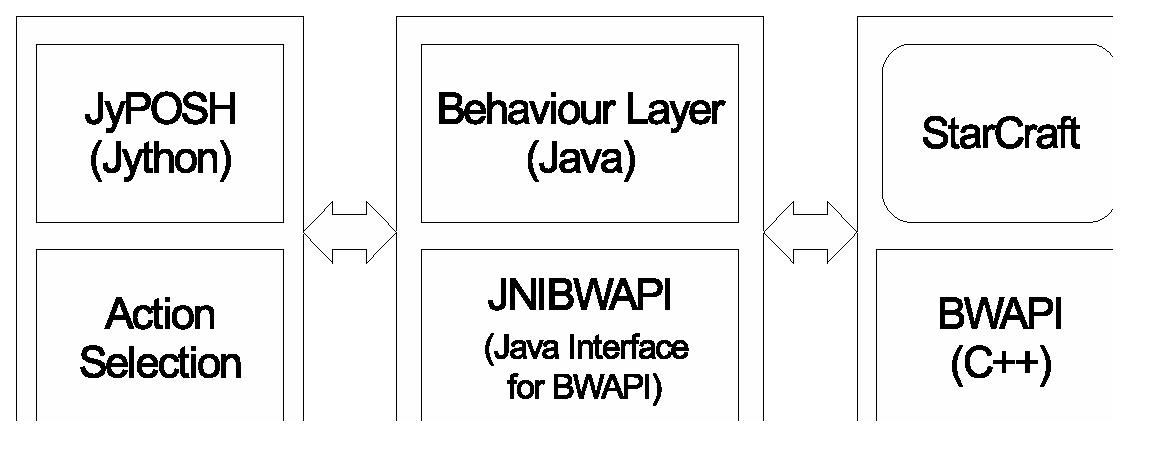
\includegraphics[scale=0.5]{AIArch}
    \caption{The architecture model for the StarCraft BOD AI. \protect\cite{davies2012}}
    \label{fig:AI-Architecture}
\end{figure}

The architecture is slightly more complicated than it needs to be, but Davies had trouble linking the python of POSH to the C++ used by BWAPI, so Java is used as an intermediary. Simplifying the architecture of the project now would require a major re-write and possibly a re-implementation of POSH in C++. This is outside the goal and scope of this project and in no way necessary, as long as JNIBWAPI remains up-to-date with BWAPI.

\label{LitSrvyClass}
The Java behaviour library of the agent is implemented as a collection of managers, which split the behaviours into correlated sub-sections. The decomposition Davies chose appears effective and his reasoning is solid.  Most of the behaviours and the action patterns are specific to the Zerg race, and as mentioned above, the other races do play quite differently. However, the base mechanics of the game (resource gathering, construction, research) are nearly identical between races and it is these areas I will look to generalise.

\section{Possible Ideas for Expansion}
This section covers various AI strategies and techniques that have been applied StarCraft and offers some opinion on their applicability for improving the agent's performance.

\subsection{Unit Micro-management Strategies}
\label{LitSrvyMicro}
Unit micro-management (micro) refers to the low-level control of units; how the units are positioned, what the units attack, and how the units attack \cite{TLMicro}.
The micro of Davies' agent is relatively simple compared to some other examples. There is a single army that moves towards the enemy's base. Each unit prioritises visible enemies based on their type and how far away they are. Each unit will then attack the unit it calculates to have the highest priority. While simple, this can be effective in some situations. It does have problems, units don't make use of any abilities they possess and units don't consider their position, so a weak ranged unit can end up in melee range. There are other works that show possible paths for improvement.

\subsubsection{Potential Fields}
Adapted from an idea in physics, this is where individual entities in the game are given an attractive or repulsive force. So units are attracted to weaker units while being repulsed from stronger or more dangerous units. Units can also be affected by changes in their own circumstances, perhaps retreating while under fire. The advantage of potential fields is that a single function can control lots of units, however the strength of the forces involved must be figured out manually and carefully considered to avoid units becoming stuck in local maxima. Genetic algorithms have been used to reduce the workload needed to optimise the values \cite{rathe2012micromanagement}. The Berkeley Overmind \cite{BerkeleyOvermind} implemented potential fields to such success that it was able to beat an ex-professional player \cite{OvermindArticle}. There are also an open source implementation available \cite{AIBot}.

\subsubsection{Monte-Carlo Planning}
Planning is usually associated with large scale strategy, due to its time cost and the large search space of micro-management. \citeasnoun{zheusing} have applied it to the micro-management of units using a Monte-Carlo planning method. Monte-Carlo methods rely on entering random samples into a simulation and analysing the results \cite{MonteCarlo}. Wang et al created a simulation of the game state and then evaluated several predefined stochastic plans. They tested their AI in game and an imbalanced scenario (their AI was at a disadvantage) and it was able to beat beginner players and the original AI with some consistency, though was still beaten by an expert. This does show some potential for planning at a micro level. However, plan evaluation must be weighted manually and the simulator is limited to a few types of units and a small environment. It is unclear if this method could be scaled to a full game, as they have concerns about simulator speed .

\subsubsection{Bayesian Modelling}
There is a project that focuses on using Bayesian models for all aspects of a StarCraft AI \cite{synnaeve2012bayesian} which includes unit control \cite{synnaeve2011bayesian}. This uses the distribution of game elements to decide what to do with a unit next. Units receive tactical goals as sensory inputs and maintain a finite state machine for different modes (attacking, defending, etc.). It uses re-enforcement learning to build its probability tables and succeeded quite well in trails against both the original AI and against winners of the 2010 AIIDE competition. Their implementation is available open source.

\subsection{Macro-management Strategies}
Macro-management (macro), as used in computer gaming, is a term for the economic or large-scale strategy of the player. For StarCraft, this covers resource collection and spending; the decision on what buildings or units to build. Davies' agent is quite effective on the resource collection side, but is very restricted on the 'what to build' side. Its strategy is very rigid and doesn't adapt to the enemies actions, which is a key part of successful StarCraft play. Improving and generalising his work will require creating several strategies, and should look into making them adaptable. There is work done in StarCraft in this area.

\subsubsection{Micro Focus}
Safadi and Ernst \cite{safadi2010organization} take the interesting position that a agents macro strategy is fairly unimportant. Their view is that planning and pattern recognition is something humans excel so well at that an agent couldn't hope to match it, the agent would require a database of possible strategies which would require continuous updates as the meta-game evolves. Instead the agent should play to it's advantages in the multi-tasking area; 300 unique action per minute is considered the average for StarCraft professionals, but it would be trivial for a computer to match and beat that. They did have some success and this is comparable to how the Berkeley Overmind succeeds. However, StarCraft units generally have a "Rock Paper Scissors" dynamic; they are strong against some units and are countered by others. Effective unit-level play needs effective unit choice otherwise it can be easily exploited.

\subsubsection{Planning}
There are many replays of StarCraft games publicly available \cite{Replays}, some of which are of high level play. Using BWAPI, it's possible to retrieve lots of data from these replays and data mine the results. There are several papers that do this and use the data to create Bayesian models of what the opponents are likely to be doing \cite{synnaeve2011bayesian,hostetler2012inferring,weber2009data}.  This has the advantage that the agent gains expert-level knowledge without designers needing to know expert strategies. Planning and prediction are popular areas in the StarCraft AI field, probably due to the availability of vast amounts of completed game data. The main strategy in StarCraft revolves around predicting and countering the opponents high-level decisions, so a successful agent does need to react in someway to what it thinks its opponent is doing.

\subsubsection{Case-based Reasoning}
\citeasnoun{certicky2013case} implemented a cased-based reasoning (CBR) method to determine which units to produce. CBR is a cyclical process where there is a databases of problem cases with solutions. For each problem, a case is chosen that best fits. The solution is adapted to fit the current problem and if it works it is added back to the database as a new case. Certicky constructed cases based on the ratios of units that the opponent has and the solutions are the recommend ratios for the agent's army. This process has the potential to be useful, but it needs quite a bit of expert knowledge about common army ratios and their counters. Additionally, this relies on good scouting and accurate information, if the agent picks the wrong case it could be disastrous. This method is perhaps a simpler incarnation of the Bayesian modelling methods discussed, and it could be a good starting point for an adaptive strategy.

\chapter{Requirements}
This chapter covers the basic requirements specification that was followed for the project.

\section{Functional Requirements}
\begin{itemize}
\item A POSH plan must be created that can control a Protoss agent:
    \begin{itemize}
    \item{The agent must be able to gather resources as the Protoss}
    \item{The agent must be able to create Protoss units and buildings}
    \item{The agent must be able to attack the enemy as the Protoss}
    \end{itemize}
\item A POSH plan must be created that can control a Terran agent:
    \begin{itemize}
    \item{The agent must be able to gather resources as the Terran}
    \item{The agent must be able to create Terran units and buildings}
    \item{The agent must be able to attack the enemy as the Terran}
    \end{itemize}
\end{itemize}
\section{Non-Functional Requirements}
\begin{itemize}
\item{Refactoring the behaviour library should not negatively affect the existing Zerg agent's performance.}
\item{The behaviour library should avoid race specific behaviour where possible}
\end{itemize}

\section{Inherited Non-Functional Requirements}
\citeasnoun{davies2012} specified several non-functional requirements that are still relevant to the project.
\begin{itemize}
\item{The application must use the BWAPI interface for communicating with StarCraft}
\item{The agent must be able to work in the latest version of StarCraft: Brood War}
\item{The AI should be designed in a modular and extensible fashion, to allow for future developments and improvements}
\item{The application must be able to run at a minimum of speed of a frame every 42ms, so not to slow down the game, as specified by the current AIIDE rules.}
\item{All relevant AI behaviours must be accessible to the POSH action selection mechanism}
\end{itemize}


\chapter{Design}
This chapter covers the design work done for the project, including an overview of the initial class structure of the behaviour library, the changes needed to generalise the behaviour library and the process used to effect the generalisation.

\section{Generalisation}
Behaviour Oriented Design encourages behaviours to be implemented in an object-oriented style \cite{bryson2003behavior}. So generalising Davies' behaviour library should be done in an object-oriented style. In this style, a super-class is created by extracting common attributes and methods from more specialised classes. The specialised classes then become sub-classes of the new class. Because Davies' library has no behaviour for other races, this project will apply the process backwards; using the already implemented behaviour as a base and sub-classing parts that can't be applied to the other races.

\section{Initial Behaviour Library Structure}
The behaviour library is the main place that needs to be refactored and generalised. As mentioned in section~\ref{LitSrvyClass}, the behaviour library is decomposed into eight classes which manager the different areas of the game. Davies' class diagram can been seen in figure~\ref{fig:SimonClassDia} and he outlined the class thusly:
\begin{description}
\item[Resource Manager]{Senses for actual and predicted resource counts, as well as reserving resources for future building construction.}
\item[Unit Manager]{Allows the selection of specific unit types. Mostly used by other managers.}
\item[Worker Manager]{Keeps track of workers and holds the behaviour for collecting minerals and gas. Used by the building manager for accessing workers for construction purposes.}
\item[Intelligence Manager]{Holds a knowledge base of enemy locations, and sends units to gather intelligence on enemy positions.}
\item[Building Manager]{Allows for construction of new buildings. Calculates viable building locations, and also holds senses for which buildings are currently possessed by the player.}
\item[Production Manager]{Behaviours for the creation of new units.}
\item[Upgrade Manager]{Behaviours for researching upgrades for units.}
\item[Military Manager]{Behaviours for the movement of military forces. This includes attacking the opponents base, retreating, and contains a list of priority targets.}
\end{description}

The immediate design work was to analyse each class's code and identify methods that could be generalised or that were already general. Any methods that are too specific would be moved into a race specific sub-class of the manager.

\begin{figure}[h]
    \centering
    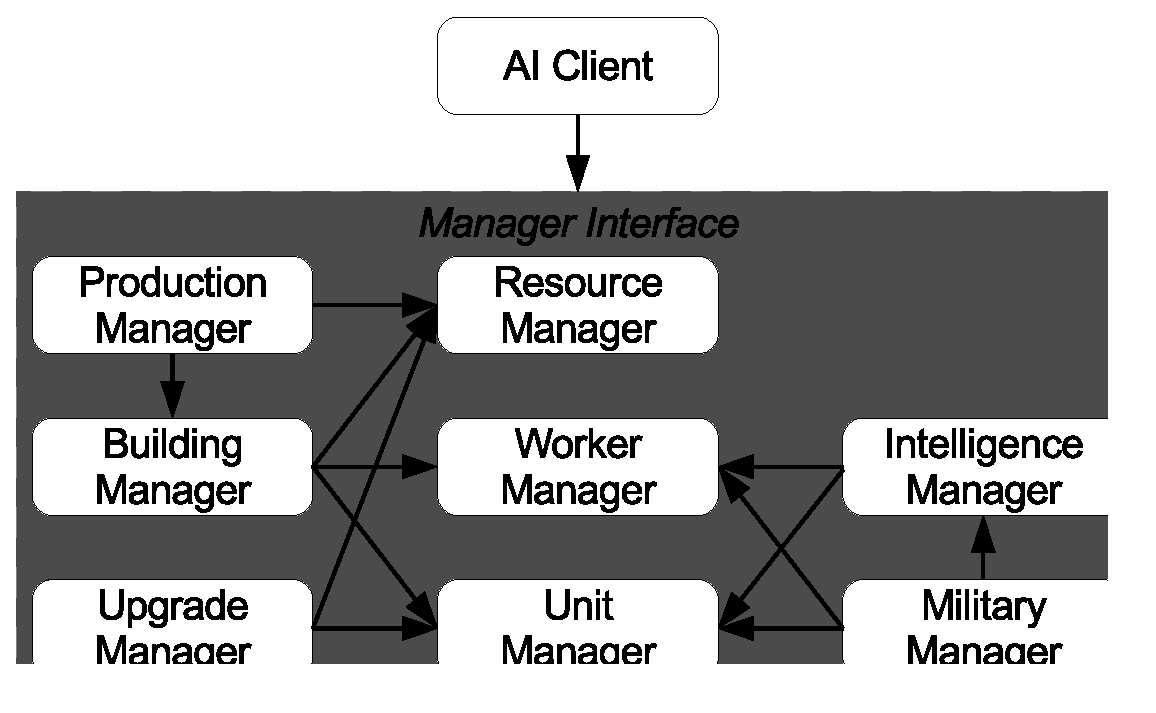
\includegraphics[scale=0.5]{OrigClassDia}
    \caption{Davies' class diagram that shows the Managers used for the categorising the different behaviours. The connections between the managers shows which classes call behaviours from other managers.\protect\cite[Fig.~3.2]{davies2012}}
    \label{fig:SimonClassDia}
\end{figure}

\section{Behaviour Library Structure Changes}
\subsection{Initial Design}
After statically analysing the code, it was found that half the classes could be fully generalised or were already general enough to not need any modification at all.

These classes were:
\begin{description}
\item[Resource Manager]Every race competes for the same resources and they each handle resources in the same way.
\item[Unit Manager]The methods in this class are already parameterised by unit type.
\item[Worker Manager]Each race uses workers and gathers resources in nearly the same way. Generalisation is mostly changing method and variable names.
\item[Intelligence Manager]Each race receives the same information about the world. Generalisation just needs to parameterise scouting.
\end{description}

The remaining classes were sub-classed in a general way, which can be seen in figure~\ref{fig:GeneralStructure}. During the initialisation of the AI client, the appropriate sub-class will be created, based on what BWAPI reports about the player's selected race.

\begin{figure}[h]
    \centering
    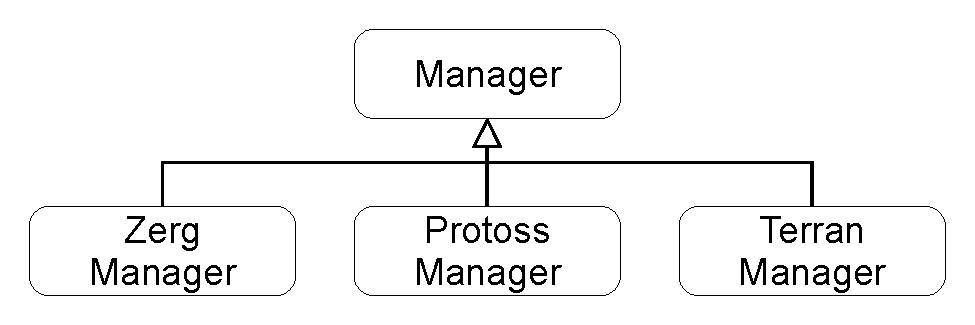
\includegraphics[scale=0.5]{GeneralStructure}
    \caption{The general class structure used when methods couldn't be generalised.}
    \label{fig:GeneralStructure}
\end{figure}

\subsection{Iterative Design Process}
After this initial design work, I proceeded with implementation. The iterative development methodology used in BOD means the design is repeatedly modified as work progresses. The process that was followed for implementation was a very slightly altered version of the BOD development methodology which went like this:
\begin{itemize}
\item{Choose a behaviour of the Zerg agent.}
\item{Implement and test the behaviour for the other races.}
\item{Evaluate race specific behaviours, looking for common patterns that could be made general.}
\item{Implement and test the generalisation.}
\item{Repeat the process.}
\end{itemize}

 This differs from BOD in that there is less focus on revising the specification, more on getting the other races capabilities up to par with the Zerg. The Zerg agent was used as the specification for the other races agents, so while revisions weren't avoided, they were not the focus of the process.

\subsection{Final Class Structure}
The final class structure of the behaviour library can be seen in figure~\ref{fig:ClassDia}. The race-specific sub-classes have been hidden as they increase the complexity of the diagram without really adding any information. The only change to the structure that came up during implementation was to the intelligence manager. It was found to be better to split the scouting control(moving the unit around) into its own class and have the intelligence manager start the scouting. This allowed for race specific scouting behaviour without code duplication.
\begin{figure}[h]
    \centering
    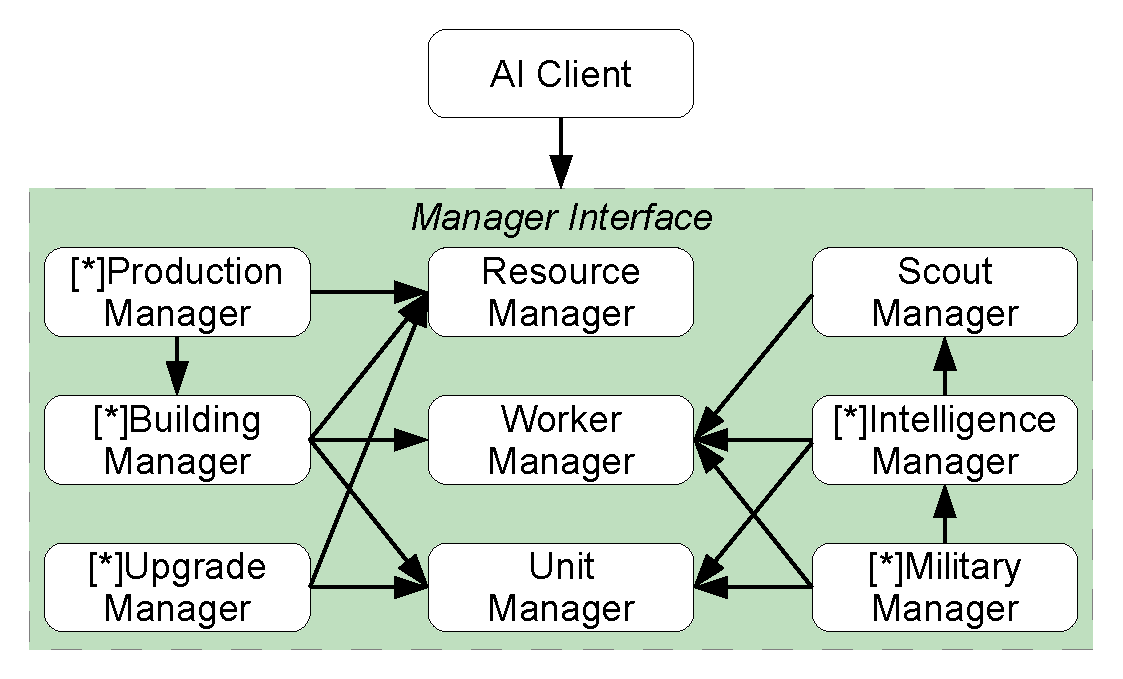
\includegraphics[scale=0.5]{ClassDia}
    \caption{The final class structure of the behaviour library. Classes with a ``\lbrack*\rbrack'' in their name have race specific behaviour in sub-classes in the style of figure~\ref{fig:GeneralStructure}.}
    \label{fig:ClassDia}
\end{figure}

\chapter{Implementation}
\label{Implementation}

\section{Behaviour Library Generalisation}
This section covers some of the work done generalising the Java behaviour library.
\subsection{API Issues}
\label{APIIssue}
This subsection explains the issues experienced by updating the external libraries that the AI uses and details how they were overcome.

BWAPI and JNIBWAPI had both released newer version since \possessivecite{davies2012} work. It was decided to update the project to use these newer versions as they offered bug fixes and the JNIBWAPI update exposed more BWAPI functionality. The update went fine, and seemed to be without issues. It was then noticed that workers would not act on any command they were given, unless it was sent during a game tick call.\footnote{A common feature of real-time games. This is a function called regularly that will perform all the computation for the game engine. For StarCraft/BWAPI the function is called gameUpdate() and gets called at ~20Hz.} Actions from POSH are called from outside the game tick and were seemingly ignored by the engine.

To solve this required the implementation of a queue in the worker manager class where a POSH action can add the order data to when it wants to tell the game to do something. Order data generally includes the type of order; the unit ID of what is being ordered; an x and y value of the location of the order, or another unit ID to perform the order on. This data is stored in a short class. When the game tick gets called, all entries in the queue are processed and the orders sent to the game.

The bug was not limited to just workers but also affected producing units and researching upgrades, so the same fix has been applied to the production and upgrade manager classes.


\subsection{Parameterisation of Building, Recruitment and Research}
This subsection explains how the building, production and upgrade managers were moved from specific behaviour methods to general, parameterised methods.

In the initial stages of the project, the main content of the race-specific managers for building, production and upgrades was methods to build specific buildings, produce specific units and research specific upgrades. An example can be seen in listing~\ref{spawnZergling}. As more of these methods were added for each race, a pattern was noticed.

The pattern is:
\begin{itemize}
\item{The progenitor unit type for the requested unit type is determined, hard-coded initially.}
\item{A free unit of the progenitor type is found.}
\item{It is checked if the necessary resources and research are available.}
\item{The action is performed.}
\end{itemize}

\begin{Code}[frame=single,language=Java,breaklines,breakatwhitespace,caption={The original method used to produce a Zergling\protect\footnote{Zerglings are the basic unit of a Zerg player's army. They are small, fast, and have a melee attack}},label=spawnZergling]
public boolean spawnZerglings(){
    for (Unit unit : bwapi.getMyUnits()) {
        if (unit.getTypeID() == UnitTypes.Zerg_Larva.ordinal()) {
            if (resourceManager.getMineralCount() >= 50 && resourceManager.getSupplyAvailable() >= 1 && buildingManager.hasSpawningPool(true))
            {
                bwapi.morph(unit.getID(), UnitTypes.Zerg_Zergling.ordinal());
                return true;
            }
        }
    }
    return false;
}
\end{Code}

Using methods provided by JNIBWAPI, it is possible to find out all the needed information just from the unit type. The code to do this can be seen in listing~\ref{produceUnit}. The important methods that allow this simplification is canMake() method provided by JNIBWAPI and the getLeastBusyUnitofType() method added to the unit manager.

canMake() has two forms in BWAPI, and it is the first that is the most valuable. The first method checks that it is valid to build that unit type; that means the necessary resources are available, the necessary research has been performed, and that there exists a unit on your roster that is the progenitor type for the passed type. The second canMake() method checks if a specific unit can make the passed unit type; so it is the correct type and it is not busy with another task.

getLeastBusyUnitofType() is needed as it is common to build multiple production units as certain races to parallelise the tasks they perform.\footnote{Production units can only perform a single task at a time, and most tasks take a long time, so it is pretty much a required tactic as the Terran and Protoss.} The method checks each unit of the passed unit type and returns the unit that has the smallest production queue, and that isn't researching anything.

\begin{Code}[frame=single,language=Java,tabsize=4,breaklines,breakatwhitespace,caption={The current method to produce any unit in the game. IntTriple is a custom type that simply contains three public integers.},label=produceUnit]
public boolean produceUnit(UnitType.UnitTypes unitType){
	int unitTypeID = unitType.ordinal();
	if( bwapi.canMake(unitTypeID) ){
		int builderTypeID = bwapi.getUnitType(unitTypeID).getWhatBuildID();
		
        Unit buildUnit = unitManager.getLeastBusyUnitofType(builderTypeID);
		
		if (buildUnit != null){
			int buildUnitID = buildUnit.getID();
			
			if( bwapi.canMake(buildUnitID, unitTypeID) ){					
				if(bwapi.getUnitType(unitTypeID).isAddon()){
					buildQueue.add(new IntTriple(IntTriple.ADDON, buildUnitID, unitTypeID));
				}
				else if(bwapi.getUnitType(builderTypeID).isBuilding()){
					buildQueue.add(new IntTriple(IntTriple.TRAIN, buildUnitID, unitTypeID));
				}
				else{
					buildQueue.add(new IntTriple(IntTriple.MORPH, buildUnitID, unitTypeID));
				}
				
				return true;
			}
		}
	}
	return false;
}
\end{Code}

\subsection{Generalising Scouting}
This subsection explains how the scouting behaviours of the AI were generalised and the reasoning behind the decisions.

The original scouting code had two types of units that it would use for scouts. Each type was managed by separate but similar methods. The aim when generalising was to merge the two methods together, preserving the functionality of both methods. The merged method also needed generalisation so that it could be applied to any type of unit. 

This has been done by maintaining a list of the currently scouting units. A ``ScoutUnit'' class was created to encapsulate all the information needed to perform the scouting. This included the unit object, the path to scout, how far along the path the unit is, and a completion handler to be called when the path has been completed. The scouting path is stored as a queue of Point\footnote{java.awt.Point: Has only two public int variables x and y} objects. As the scout reaches each location, the next location is popped from the queue. The completion handler is implemented as an interface with a single method scoutRouteCompleted(), which takes the scouts ID as a parameter (otherwise, the called object won't know which scout finished).

The implementation of this generalisation grew quite large, large enough that scouting took up a large proportion of the intelligence manager. This spurred the decision to move scouting into its own class. The intelligence manager remains the initiator and completion handler for scouts; the scout manager is envisioned as more of an internal utility class. If the scout manager handled scouting completely, it would require race-specific sub-classes, which is to be avoided as much as possible as specified in the requirements.

\subsection{Generalising the Military}
\label{MilitaryGen}
This subsection explains how the military behaviours of the AI were generalised and the reasoning behind the decisions. 

The action selection of military units requires quick reactions and a large amount of contextual information, like what units are around, what position they are in, map obstacles, etc. The correct action also depends on the type of the unit being controlled. Using POSH plans is not feasible for this as it is not fast enough and it doesn't have the fine precision needed. So this action selection has to be implemented in the behaviour libraries. 

Davies' had hard-coded the behaviour for the units used in his plan, which meant control for different unit types had to be manually added. This is somewhat desirable, as there are many units which would benefit from unique behaviour. However, it makes adding a new unit to a plan harder than it needs to be; sometimes the unique behaviour isn't essential to a unit's performance. So, the goals while generalising this class were to remove as much hard-coded behaviour as possible while being easily extendable with specialised behaviours.

Military units were organised into hard-coded lists of units of certain types. So there was a ``zergling'' list and a ``hydralisk\footnote{Hydralisks are a Zerg ground unit with a ranged attack}'' list and so on. To extended this without using individual lists for each unit type, the individual lists have been combined into a map. The keys in the map are the unit type ID and the values are the lists of units of each type. All units that are created are added to these groups (excluding buildings); units that change into other units are moved between lists; Destroyed units are removed from the lists. This simplifies the process of adding behaviours for a new unit type; all units are accessed from a central place, which can do all the maintenance for you.

After the management was generalised, the focus moved to the control. Originally, units were controlled by iterating through each unit list and sending the chosen command to each unit. The solution first tried was to just copy this functionality in the race-specific sub-classes. Apart from being bad software development practise, this was problematic as it meant control for new unit types had to be added manually, just like the original code. On the other hand, controlling all units in the same way is undesirable as different unit types often have abilities they can use or want to move and attack in a different way.

The implemented solution to this is to use the basic movement and attack behaviour for all units in the super class, while having any specialised behaviour in the race-specific sub-class. A list of ``special unit types'' is kept which indicates to the default method that it should skip the current unit type and let the sub-methods handle it. This makes it easy to add new units to POSH plans while allowing specialised behaviour where necessary.

\subsection{Small improvements}
This subsection covers small improvements made to the behaviour library.
\subsubsection{Build Locations}
The building manager maintains a list of build locations, which it chooses from when it is time to build a building. The locations were originally generated based on the locations of resources nodes near initial base building. The method needed to modified, but it was too complex. The method has been re-written to be simpler and easier to follow.

Another improvement to build locations is that when one is added, the position is checked to ensure it doesn't conflict with any existing build locations. This is needed for both the Protoss and the Terran as both would duplicate locations as they built buildings which would then create cluttered bases.
\subsubsection{Resource Reservation}
The original resource reservation system simply an integer variable that could be set when a behaviour needed to reserve some resources. Multiple resources reserving at the same time just wasn't feasible because while behaviours could simply increase the reservation instead of setting it, the behaviours are no longer running by the time the task is performed and the resources consumed.

The solution implemented to solve this is to pass an integer ID along with the reservation amount. Then when the resources have been consumed, the reservation with the chosen ID can be cleared. This makes simultaneous reservations easier to deal with, but it doesn't solve the problem of not knowing when to clear the reservation. Reserving resources is only done when building as there is a delay between the command and the resources being spent. Any other time resources are spent, it happen instantly. By using the worker unit ID as the reservation ID, it can be identified when the resources have been spent and which reservation to clear.
\subsubsection{Impatience}
The original AI had an issue where after it destroyed the main enemy base, it wouldn't search for any extra bases that may have been built. This can result in a loss, as the enemy can rebuild its army. To counter-act this, an ``impatience'' timer has been implemented. This is a timer that waits for a certain number of game ticks, then changes the attack destination to a different base location\footnote{Most, if not all, StarCraft maps have a limited number of viable base locations around clusters of resource nodes.}. The timer is reset upon sighting an enemy. The effect of this it that if the army successfully destroys the enemy's main base, it will cycle around the map until it finds the remnant force.
\subsubsection{Expansion Locations}
A problem in the AI identified by \citeasnoun{davies2012} was that possible expansion locations were calculated on straight line distance, instead of walking distance. So bases that are close by but take a long time to walk to would be preferred over more accessible options. This couldn't be fixed at the time as JNIBWAPI did not provide the necessary functions. The updated JNIBWAPI does provide the necessary functions, so the method has been updated to make better choices.

\section{POSH Plans}
POSH plans are hierarchical plans with lisp like syntax. They are explained in section~\ref{POSHPlans}. This section details some of the POSH plan elements created or changed during the project.

\subsection{Overall Strategy}
The aim of this project is to flesh out Davies' behaviour library, so that it can be used by all races. To test that the generalisations were successful, POSH plans were created for the Protoss and the Terran. These plans followed the same general strategy that Davies' plan followed, with minor adjustments. This sub-section will outline that strategy.

\subsubsection{Initial Behaviour}
The very start of a game is identical for all races. Workers are ordered to collect minerals and new workers are produced. The first behaviour is handled automatically by the behaviour library. The second behaviour has to be outlined in the plan, and initially the Protoss and Terran copied the Zerg. As development continued, some problems were found with Davies' approach, so worker production was modified slightly(see section~\ref{workerProd}).

\subsubsection{Building a Military}
Once a decent number of workers have been amassed, and minerals are flowing in, it is time to start spending. The next goal for every race is to construct their first tier military building\footnote{Buildings in StarCraft often require other buildings to be built before they can be built. Buildings without these requirements can be called the first tier buildings.}, so that some soldiers can be recruited for defense (and eventual offense). The behaviour for Protoss and Terran is slightly different to the Zerg here because of the unique way Zerg produce units. Protoss and Terran units are produced at certain buildings. It is common to build several of these buildings during the game so that units can be produced at a faster rate. It was decided that both the Protoss and the Terran would build two of these buildings, based on basic analysis of several online build orders\footnote{Build orders in the StarCraft community refer to the initial strategy of the player, detailing the order and timings of building and production. Build orders are regularly shared on websites like \citeasnoun{TeamLiquid} and \citeasnoun{StratWiki}.}. As soon as these buildings are finished, they begin producing the basic soldier for each race.

\subsubsection{What to do Next}
At this point there are several choices on what to do next.
\begin{description}[leftmargin=1.5cm,labelindent=1cm]
\item[Research upgrades]{Units in StarCraft rarely start out at their full potential. Each race has many upgrades and technologies to research to improve certain units effectiveness. Generally, research is conducted at specialised buildings. Research takes a long time, so it is important to start early. With that in mind, that is one of the next steps in the strategy; build the correct buildings and start researching.}
\item[Expand to new bases]{It is important to continue growing the economy after the start of the game. Expanding allows for a greater resources income, which leads to a larger and stronger army.}
\item[Produce different units]{It is rarely a good idea to focus on a single type of unit. More units can be made available by building certain buildings. Which buildings to choose depends on the overall strategy.}
\end{description}
These behaviours can often be done in parallel, if the resources are available. There is also some overlap. New buildings can unlock new upgrades as well as new units. The plans created for the Protoss and Terran differ slightly from the Zerg plan; expansion happens slightly later as it costs more resources, and research buildings are built sooner because of racial differences\footnote{The Zerg have more research options in their basic buildings than the other races do.}.

\subsubsection{When to Attack}
Choosing the best army size to begin to attack is tricky. Too soon and it may not be strong enough to succeed. Too late and the enemy may be too well defend, or countered your unit choices. There isn't a good formal way to decide this, it has to be worked out via trial and error and probably should be adjusted depending on the opponent's strategy. There is a simple competence to give some variability to this, where the attack size is adjusted based on the enemies race. For example, the Protoss plan attacks later when facing a Zerg opponent, as the Zerg often have invisible units and delaying the attack allows for detection units to be produced.


\subsection{Simplified Competences}
The iterative development process outlined by BOD involves re-evaluating previous implementation after each cycle. This sub-section details the results of one such evaluation where it was noticed that some behaviours were more complicated than they needed to be at the plan level and how that was remedied.

The task of starting to gather gas is a two step process. The first a building needs to be built on the gas resource nodes. Once this building has completed, workers must be moved from other tasks to begin harvesting the gas. The original POSH plan (see listing~\ref{oldGasPOSH}) had both these steps in a competence. Due to bugs resulting from upgrading the external APIs (see section~\ref{APIIssue}), the second step of the competence would often not work, and there would be a large delay between the building being completed and workers starting to gather gas.

\begin{Code}[frame=single,language=Lisp,tabsize=4,breaklines,breakatwhitespace,caption={The original POSH competence to manage collecting gas},label=oldGasPOSH]
	(C collect-gas-competence (seconds 1.0) (goal ((gas_saturated)))
		(elements
			(
				(put-workers-on-gas (trigger ((all_extractors_completed)
					(gas_saturated 0 =)
					(has_extractor))) start_collecting_gas -1)
			)
			(
				(build-extractor (trigger ((has_extractor_saturation 0 =)
					(has_extractor 0 =)
					(mineral_count 25 >=)
					)) build_extractor 1)
			)
		)
	)
\end{Code}

The solution found for this is to move the second step directly into the behaviour library. It will never be the case that a gas extraction building is constructed without needing workers sent to it. A new feature of JNIBWAPI is an event when ever a unit is completed, so the completion of the extraction building is detected and workers are reassigned. The competence has been refactored into a drive element and an action pattern\footnote{The action pattern only has a single primitive. It is necessary as the version of POSH used cannot call action primitives from a drive element.}. The drive element can be seen in listing~\ref{newGasPOSH}.

\begin{Code}[frame=single,language=Lisp,tabsize=4,breaklines,breakatwhitespace,caption={The current POSH drive to begin collecting gas},label=newGasPOSH]
(
	; Start collecting gas
	(get-vespene (trigger (	(has_completed_spawning_pool)
							(has_extractor_saturation 0 =)
							(mineral_count 25 >=)))
		build-extractor-ap(seconds 4.0))
)
\end{Code}

A similar method was employed in the expansion building behaviour. There was one competence that would send a worker to an expansion, and then when it appeared the worker had arrived, there was another competence to tell the worker to build. This suffered the same kind of bugs as starting to gather gas, and in some cases would it result in two new base buildings\footnote{All races in StarCraft have buildings where harvested resources need to be returned, so that they can be added to the resource pool. These buildings form the core of any new base, and are referred to as base buildings.} in the same location (the worker would take too long to build, so another worker would be sent). This is a waste of resources and not really desirable.

The solution here is the same as the extractor problem. It can be detected when the worker arrives at the expansion location, so instead of waiting for the action selection mechanism to choose to build, it is done as soon as it is necessary. This speeds the process up, and reduces the behaviour to a single action pattern. Like with building a gas extractor, the actions are tied together; A worker wouldn't be sent to expand without the intention to build a new expansion.

\subsection{Improvements to Worker Production}
\label{workerProd}
During testing, it was noticed that Davies' plan produces workers quite frequently. The plan has multiple drive elements to trigger worker production, and because of workers low cost compared to most other units, workers get produced frequently. This isn't a massive problem; workers are used to collect resources so as the game progresses the rate that resources are spent on workers is outpaced by the rate that those workers collect resources. However, it does delay the production of military units, both by consuming resources and by occupying space in the recruitment queue. It can be fixed by adding more restrictions to recruitment of workers, but the distribution of the activation across several drive elements makes this harder than it needs to be. The Protoss and Terran plans attempt to improve this.

\begin{Code}[frame=single,language=Lisp,tabsize=4,breaklines,breakatwhitespace,caption={A competence to control the production of worker units at different stages of the game.},label=workerPOSH]
(C worker-production-competence (seconds 1.0) (goal ((game_over) (drone_count 50 >)))
	(elements
		(
			(build_workers_late_game(trigger (
										(expansion_count 1 >=)
                                        (zealot_count 13 >)
										(drone_count 51 <)
										(mineral_count 50 >=)
										(supply_available 2 >)))
				train_probe -1)
			(build_workers_mid_game(trigger (
										(zealot_count 9 >)
										(drone_count 26 <)
										(mineral_count 50 >=)
										(supply_available 2 >)))
				train_probe -1)
			(build_workers_initial (trigger (
										(drone_count 11 <)
										(mineral_count 50 >=)
										(supply_available 2 >)))
				train_probe -1)
		)
	)
)
\end{Code}

These plans group worker production into a single competence with each element covering a different stage of worker production. Listing~\ref{workerPOSH} shows the competence used by the Protoss plan. At the start of the game, worker production has very little constraints. This is so enough workers are produced to create a good resource income. Production is then halted until some military units have been produced. This provides some protection against early attacks by the opponent. It also allows resources to build up, that way more resource expensive behaviours are likely to fire. Worker production is constrained again in the late game until an expansion is built, as increasing the amount of workers at a resource node gives diminishing returns. Other constraints are similar to the mid game because the calling drive element is low priority. As the game progress, higher priority drive elements become available, so worker production is chosen less, so more constraints aren't needed. The higher priority drives are effectively implicit constraints on this behaviour.



\chapter{Results}
To measure the performance of agents, they have been tested in matches against existing StarCraft AI, mainly the official AI provided by Blizzard.

The tests will use the same metrics that \citeasnoun{davies2012} used, which are really the only quantifiable metrics available. Using them will make it easier to compare with Davies' work. Davies' used two metrics, the outcome of the match and the percentage difference between the final scores of both players. Both metrics are calculated by the game.

The outcome of a match can either be a win or a loss and occurs when one player has lost all their buildings. The score is the total of three scores, the unit score, the building score and the resource score. The unit and building scores are calculated on the amount and the types of units/buildings produced and destroyed (more powerful/expensive units are worth more). Destroying a unit or building is usually worth double the score from producing that unit. The resource score is the total resources collected.

The win/loss metric is of obvious importance when deciding if an agent was successful, the difference in scores is useful to show \textit{how} successful an agent was. A small difference in score implies that the match was close; neither side had too much of an advantage. A large difference shows the opposite.

The tests will be split between two maps, to see if this affects performance. The maps used will be Azalea, which Davies used for his tests, and TBD because reasons.

PUT TABLE HERE

ANALYSIS HERE


\chapter{Discussion}


\section{Behaviour Oriented Design}
This project made use of both the architecture and the methodology of BOD. The elements are explained in more depth in section~\ref{BOD} and by \citeasnoun{bryson2003behavior}.

The architecture of BOD has two layers, a behaviour library and POSH plans for action selection. This structure has been beneficial for this project. The conceptual distinction between behaviours and action selection encourages modularity and generality, which made the task of extending the behaviours much easier. Because any behaviours that can be called from POSH plans could be called at any point, robustness and some generality is favoured during implementation.  POSH plans allow for the rapid creation and modification of elements, which fits the iterative development methodology well.

The development methodology is a generic iterative model, with a focus on refactoring and frequent testing. It is useful as it focuses effort on small areas, which influences the implementation towards modularity and reduces the amount that needs to be tested. It also simplifies debugging, by reducing the scope of where a bug can occur.

Frequent testing is useful when the complexity of agents or the environment is high, like in StarCraft. There are too many interactions and variables, so they can't be completely predicted before hand and assumptions have to be made. Frequent testing can correct these assumptions before they have a large effect on the code.

The refactoring process is arguably the most important part of the BOD methodology. Before implementing a new part of the specification, the specification and the existing implementation is evaluated, to check for behaviours that are too complex, that would work better as a different element. Often when implementing, the desired behaviour arises from hacks and intuition. Looking at code after some time can give a developer a different perspective and allow them to pick out an elegant solution. This leads to the code being easier to understand and to extend.

\section{POSH}

POSH plans are a useful tool. They are quick to set up, and provide a simple way to direct complex behaviours. However, they do have their limitations.

\subsection{Problems with Development}
Developing POSH plans is not as easy as it could be. It isn't overly difficult but the lack of a good development environment and debugging tools can take time away from actual development work. There are two ways to develop POSH plans, by using a text editor or by using the ABODE editor \cite{abode}. ABODE does provide a graphical visualisation of plans, however it is still beta software so it suffers from bugs, it doesn't have any debugging features or code completion, and it has a lack-luster user interface. It is usually easier to edit the plans in a text editor, at least at first. Plans are in single files, so if one has a lot of elements it can be difficult to organise.  The syntax can also cause issues when developing in a text editor. It has similarities to Lisp, with lots of parenthesises which can easily be misplaced.

The editing issues are very minor quibbles, but the lack of proper debugging tools is a bigger problem. Debugging of the plans is limited to console output, which gets quickly overloaded once plans reach a reasonable size. This output is verbose without being particularly informative, drives are ``inhibited or not ready'', for example, without any information as to why. It would be useful to know which kind of failure it is, inhibition or unreadiness. When inhibited, the duration of the inhibition could be displayed and when the element isn't ready the trigger that failed could be displayed. The ability to set break points and step through the plan execution would make it easier to check this information and allow a developer to quickly get to grips with a plan's flow.

\subsection{Primitive Parameterisation}
In the python side of the behaviour library there are many action primitives and senses which cannot be generalised due to the way POSH works. Elements in POSH plans do not accept parameters, so primitives must be explicit about what they do (see listing~\ref{behaviours}). Because the underlying behaviour has been generalised, there is a lot of code duplication in the python behaviour modules that isn't really necessary. While this doesn't really affect an agents performance, or even the complexity of an agents plan (an agent will only use a small fraction of available primitives), it feels like ``code smell''\cite{Emden02javaquality}, it could hamper future development.

One way to solve this problem would be to move the action selection into the behaviour library. Have an action ``choose next building'' and then other behaviours can use that next building accordingly. This would require no changes to POSH and is a recommended way to solve this issue \cite{bryson2003behavior}. However, it is a complex task, probably one that deserves its own project. Even with this kind of mechanism in place, the ability to sense and obtain specific buildings, units or research would still be desirable, to allow for plans to act outside of the shared action selection.

A different way to solve this is having parameters passed with behaviours. The main effect of this would be to reduce the number of behaviours and code duplication needed. This would also give behaviours more flexibility and reduce the busywork needed to extend identical behaviours to similar objects.

\begin{Code}[frame=single,language=Python,tabsize=4,breaklines,breakatwhitespace,caption={A small selection of similar behaviours to build different buildings.},label=behaviours]
def build_bunker(self):
	return self.agent.BWBot.bot.buildingManager.buildBuilding( UnitTypes.Terran_Bunker )

def build_engineering_bay(self):
	return self.agent.BWBot.bot.buildingManager.buildBuilding( UnitTypes.Terran_Engineering_Bay )

def build_factory(self):
	return self.agent.BWBot.bot.buildingManager.buildBuilding( UnitTypes.Terran_Factory )

def build_missle_turret(self):
	return self.agent.BWBot.bot.buildingManager.buildBuilding( UnitTypes.Terran_Missle_Turret )

def build_science_facility(self):
	return self.agent.BWBot.bot.buildingManager.buildBuilding( UnitTypes.Terran_Science_Facility )
\end{Code}


Moving complex action selection into the behaviour library feels a bit like re-inventing the wheel. There is already action selection happening in POSH, why duplicate the effort? The reason to do so at the moment is because POSH is limited, probably intentionally. There is an interplay in the BOD methodology over where complexity should be, the plans or the behaviour library. The BOD methodology encourages developers to strike the best balance here via rapid iteration, frequent testing, and the repeated re-evaluation of what has been done. POSH is a tool in the methodology to direct a developer's thinking usefully about the best way to create an agent. So by limiting what can be expressed in a POSH plan, a developer is directed to moving complexity into the behaviour library\footnote{Conversely, an emphasis on modularity encourages the simplification and reduction of behaviours, pushing the complexity towards the plans}.

Using the architecture of BOD could be a good way to introduce non-programmers to AI concepts by letting them easily build their own. Once you understand the aggregates of POSH -- something made easier with a graphical representation, like ABODE -- creating plans becomes a matter of piecing together the building blocks; the complicated implementation is kept hidden from the end user. This project attempted to facilitate a situation like this in the future by including behaviours for as many in-game actions as possible. Whether this was successful, and if BOD could be used as a learning tool, would need to be tested in future work.

\section{State of the Behaviour Library}
This project has been successful in its goal of extending Davies' behaviour library. The Java code has been refactored into a generalised structure, which brings together shared behaviours while still allowing for specialised (race specific) behaviour to be added when needed. The jython behaviour modules have also been extended so that they have actions and senses for every building, unit, and research available for every race in the game. There are also POSH plans that have been developed to showcase agents of the other races.

At this point, the library provides a solid base on which to build or try out new AI strategies in the StarCraft environment. It provides the fundamental behaviours required to perform in a game of StarCraft\footnote{Attacking and defending, resource gathering, exploration and expansion, and construction, unit production and research} for all races, and they are exposed in a reasonable way as POSH plan primitives.

\section{Remaining Issues and Future Work}
There are still areas of the library that should be worked on and expanded, more advanced behaviours to be added, and maintenance to be done. This section covers some of them.

\begin{itemize}
\item{The BWAPI library and related projects are still under active development. Before this project began, the main library had released a major version (from 3.7 to 4.0) and during development JNIBWAPI was also updated. Because of issues experienced updating at the start of development (see section~\ref{APIIssue}), the project was not updated to these new versions. However, the new versions do make some major changes and fixes, so should be merged at some point.}
\item{The are a few advanced behaviours missing from the library.
    \begin{itemize}
        \item{There are no behaviours to load or unload units from flying transport units. These actions are useful for sneak attacks and for expanding to normally inaccessible areas of the map, so they should be added at some point.}
        \item{There are no behaviours to handle the Terran's movable buildings (several Terran buildings can take off and land somewhere else). It is a common tactic to use this feature to ``wall off'' the starting base as a defensive measure, where a movable building acts as a gate. Outside this use case, this is a pretty rare tactic, so perhaps only the walling off behaviour is needed.}
        \item{The Zerg have a building that has two parts, which allows instant travel from one end to the other. It is possible to build one end of this building currently, but building the other end doesn't fit into the current construction system and determining the best location to build it presents its own challenges.}
    \end{itemize}}
\item{Agents need better ways to adapt their strategy. A simple production-based system would be a good place to start with this, where if the opponents have certain buildings or units, the agents adapt accordingly. This should be implementable in the current system, the plan developed for the Protoss has a primitive version of this where attacks happen earlier or later depending on the opponents race. To extend it would just need some scouting improvements\footnote{Currently, scouts are only used to locate the enemy. Scout routes would need to be adjusted to give the most information possible.} and more senses; there are guides available to explain specific counter-tactics \cite{StratWiki}.}
\item{The library needs better unit micro-management. Several possible methods were outlined in section~\ref{LitSrvyMicro}, probably the best candidate for future improvements would be potential fields\footnote{Where units move and attack based on the gradient of their location. Other entities in the game have attractive or repulsive forces based on their state.}. The currently unit control acts in a similar way to a potential fields; each enemy unit has a priority based on its type and distance from the current unit. By taking other factors into account, like the health of units and how much damage the current unit can do, this could be converted into a better approximation of a potential field without major restructuring.}
\item{Advanced unit control is missing for most units. Unless the unit was used in one of the provided plans, no additional behaviour was added, so most units won't use their abilities. This is something that should improve overtime as more plans are developed, even if better micro-management is not added.}
\end{itemize}









%%
%% Now we are back to the standard project contents that you should include
%%

\chapter{Conclusions}
%% Uncomment this to include a separate tex file wih the conclusion contents
%\include{conclusion.tex}

This is the chapter in which you review the major achievements in the
light of your original objectives, critique the process, critique your
own learning and identify possible future work.

\bibliography{LitRef}

\appendix

%%
%% Use the appendix for major chunks of detailed work, such as these. Tailor
%% these to your own requirements
%%

\chapter{Design Diagrams}

\chapter{User Documentation}

\chapter{Raw results output}

\chapter{Code}

%%
%% NOTE that for this to typeset correctly, ensure you use the pdflatex
%%      command in preference to the latex command.  If you do not have
%%      the pdflatex command, you will need to remove the landscape and
%%      multicols tags and just make do with single column listing output
%%

\begin{landscape}
\begin{multicols}{2}
\section{File: yourCodeFile.java}
\lstinputlisting[basicstyle=\scriptsize]{yourCodeFile.java}
\end{multicols}
\end{landscape}

\end{document} 